\chapter{Towards Learning in Linear Models}

\section{Advanced Problem Formulations (Slides)}

The below are a list of major subject areas in NeurIPS \footnote[1][]{As of 2024, when the slides were created.}:
\begin{itemize}[noitemsep]
    \item Supervised, Unsupervised or Semi-Supervised Learning:
          \begin{itemize}[noitemsep]
              \item Few-shot Learning
              \item Transfer Learning
          \end{itemize}
    \item Unsupervised Learning:
          \begin{itemize}[noitemsep]
              \item Density Estimation
              \item Clustering
              \item Dimensionality Reduction
          \end{itemize}
\end{itemize}


\subsection{Few-shot Learning}

In supervised learning, let us define the notation:

\noindent Let our feature vector (which is our input space) be defined by
\begin{equation}
    x \in \R^n
\end{equation}

\noindent Let our output labels be defined by
\begin{equation}
    y \in \R^m
\end{equation}

\noindent  Assume our dataset is i.i.d distributed and  $K >> n$, it is defined as
\begin{equation}
    \mathcal{D} = \{(x^{(i)}, y^{(i)})\}_{i=1}^K
\end{equation}

Our learning objective is to find the minimum error from our loss function $\mathcal{L}$.
\begin{equation}
    \min_\theta \left[ \mathcal{L}(f^\theta(x),y) \right]
\end{equation}

In the case of \textbf{few-shot learning}, a technique in ML where a model learns to perform a task proficiently with only a limited amount of training data. We do not have the luxury of $K \gg n$ and so our model must learn to generalise well, quickly.


\begin{itemize}[noitemsep]
    \item When $K = n$:
          \begin{itemize}[noitemsep]
              \item \textbf{n-shot learning}: Trains with $n$ examples per class.
              \item Example: With $n=3$, learn to recognise animals like cats, dogs, and birds from three images each.
          \end{itemize}
    \item When $K = 0$:
          \begin{itemize}[noitemsep]
              \item \textbf{zero-shot learning}:\footnote[][]{Very popular with Large Language Models (LLMs) and also known as zero-shot prompting in this case.} Infers classes with no examples, using descriptions.
              \item Example: Identify an animal as a mammal based on descriptions of mammals being warm-blooded with hair.
          \end{itemize}
    \item When $K = nc$:
          \begin{itemize}[noitemsep]
              \item \textbf{n-way c-shot learning}: Trains with $c$ examples from each of $n$ classes.
              \item Example: In a 5-way 2-shot scenario, classify fruits like apples, oranges, bananas, grapes, pineapples from two images each.
          \end{itemize}
\end{itemize}


\subsection{Transfer Learning}

Transfer learning is a machine learning technique where a model trained on one task is re-purposed on a second related task. Let us define two datasets, $\mathcal{D}$ and $\mathcal{D}'$:

\begin{align}
    \mathcal{D}  & = \{(x^{(i)}, y^{(i)})\}_{i=1}^N \quad \text{where } x^{(i)} \in \mathbb{R}^n, y^{(i)} \in \mathbb{R}^d        \\
    \mathcal{D}' & = \{(x'^{(i)}, y'^{(i)})\}_{i=1}^{N'} \quad \text{where } x'^{(i)} \in \mathbb{R}^n, y'^{(i)} \in \mathbb{R}^d
\end{align}

We then define the functions used in transfer learning :\footnote[][]{Bear with the difference in notation here: the notes use $\phi$ to represent the feature extractor instead of $g$.}
\begin{align}
    g^\omega & : \mathbb{R}^n \rightarrow \mathbb{R}^l \\
    h^\kappa & : \mathbb{R}^l \rightarrow \mathbb{R}^d \\
    f^\theta & : \mathbb{R}^l \rightarrow \mathbb{R}^m
\end{align}

The function $g^\omega$ represents a feature extractor that maps input features from $\mathbb{R}^n$ to a latent space $\mathbb{R}^l$. The function $h^\kappa$ is a task-specific classifier or regressor for the old task, mapping the latent features to outputs in $\mathbb{R}^d$. The function $f^\theta$ is a classifier or regressor for the new task, also mapping the latent features to outputs in $\mathbb{R}^m$. \bigskip

The learning process in transfer learning typically involves two main steps:

\begin{enumerate}
    \item Pre-training on the old dataset $\mathcal{D}$:
          \begin{equation}
              \min_{\omega, \kappa} \mathbb{E}_{\mathcal{D}}[L(y, h^\kappa(g^\omega(x)))]
          \end{equation}
          This step involves optimising the parameters $\omega$ and $\kappa$ to minimise the expected loss $L$ on the old dataset $\mathcal{D}$, effectively training the feature extractor $g^\omega$ and the old task classifier $h^\kappa$.

    \item Fine-tuning on the new dataset $\mathcal{D}'$:
          \begin{equation}
              \min_{\omega, \theta} \mathbb{E}_{\mathcal{D}'}[L(y', f^\theta(g^\omega(x')))]
          \end{equation}
          In this step, the feature extractor $g^\omega$ is further optimised along with the new task classifier $f^\theta$ to minimise the loss on the new dataset $\mathcal{D}'$. The parameters $\omega$ are fine-tuned to adapt to the new task, leveraging the feature extraction capabilities learned from the old task.

\end{enumerate}

\subsection{Density Estimation, Clustering and Dimensionality Reduction}

Assume we have an unsupervised learning setup, with $x \in \R^n$ and our dataset $\mathcal{D} = \{ x_1, x_2, \ldots, x_K \}$ where data is i.i.d and  $K \gg n$.

Notes:
\begin{enumerate}
    \item  \textbf{Density Estimation} is to estimate the probability density function (pdf) of the data distribution.
    \item  \textbf{Clustering} is to find a way to group data points as clusters. We typically first estimate how many clusters exists, then try to fit assign points to the clusters.
    \item \textbf{Dimensionality Reduction} involves finding latent factors and/or associations in the data. Even though though the spacec of the data is large, the effective dimensionality of the problem is small. For example, we can visualise the MNIST dataset of handdrawn digits from 1-10 in a 2D space with t-Distributed Stochastic Neighbor Embedding (t-SNE) in Figure \ref{fig:mnist-tsne}.

          \begin{figure}[h]
              \centering
              \begin{subfigure}[b]{0.45\linewidth}
                  \centering
                  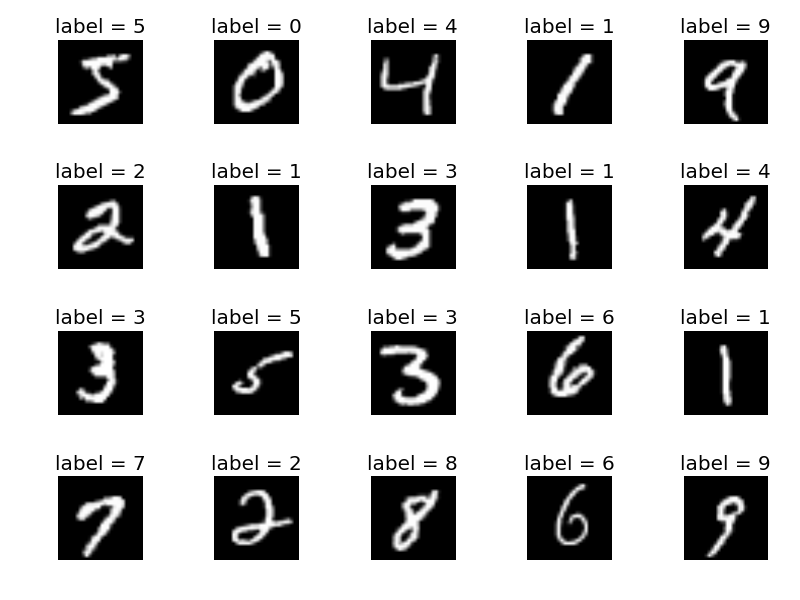
\includegraphics[width=\linewidth]{img/2_mnist.png}
                  \caption{MNIST dataset}
              \end{subfigure}
              \hfill % optional; add some horizontal spacing
              \begin{subfigure}[b]{0.45\linewidth}
                  \centering
                  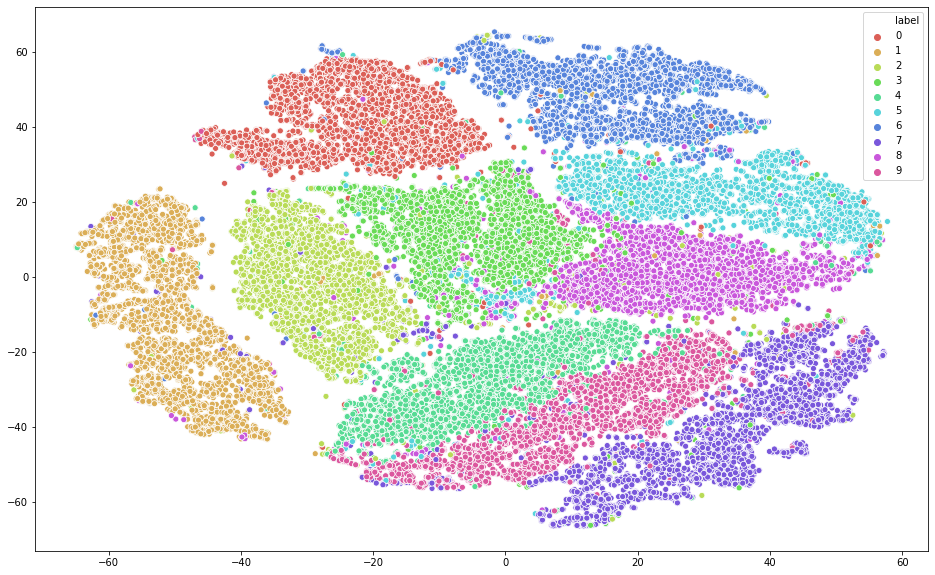
\includegraphics[width=\linewidth]{img/2_mnist-tsne.png}
                  \caption{t-SNE visualisation on MNIST dataset}
                  \label{fig:mnist-tsne}
              \end{subfigure}
              \caption{{\footnotesize MNIST dataset (dimension 10) and its corresponding t-SNE visualisation}}
              \label{fig:mnist-tsne}
          \end{figure}




\end{enumerate}


\section{Supervised Learning}
Supervised learning assumes that we have access to input-output pairs of datapoints, $(\mb{x}, \mb{y})$, with $\mb{x} \in \mathbb{R}^n$ and $\mb{y} \in \mathbb{R}^m$, forming our dataset\sidenote{The slides replaced $K$ with $N$. Notation!} $\{(\mb{x}^{(i)}, \mb{y}^{(i)})\}_{i=1}^N$.


\section{Linear Regression Model}
Assuming a domain of $\mathbb{R}^n$ and a one-dimensional co-domain, we can write our model as $f(\mb{x}) = \mb{x}^\top \mb{\theta}$. Thus we have:




\[
    \hat{y}^{(i)} = \mb{x}^{(i)\top} \mb{\theta}
\]

The goal of learning is to find $\mb{\theta}$ such that $\hat{y}^{(i)} \approx y^{(i)}$. \marginnote{You may recall linear models written as affine transformations: $y = mx + b$, where $b$ is the bias or constant term – this makes the model affine and not linear. Linear models refers to the relationship between model parameters and predictions via a linear transformation.
}



\defb{Linear Transformation}{
    A linear transformation between two vector spaces $V$ and $W$ is a map

    $$T : V \rightarrow W$$

    such that:

    \begin{itemize}
        \item $T(v_1 + v_2) = T(v_1) + T(v_2) \quad \forall v_1, v_2 \in V$
        \item $T(\alpha v) = \alpha T(v) \quad \forall v \in V \text{ and scalar }\alpha $
    \end{itemize}

}

\marginnote[-70pt]{
    \defsb{Affine Transformations}{
        Affine transformations are more general than linear transformations, because they include not only scaling and rotation, but also translations.
    }
}


Now we are faced with something interesting: $T(\mb{0}) = \mb{0}$. According to our affine transformation $f(x) = mx+b $ where $m,b \in \mathbb{R}$, we have $f(0x) = b \neq 0f(x)$, which doesn't allow us to have a bias term $b$. This is easily fixed with a straightforward modification to capture the affine transformation $f(x) = mx + b$: we just add a feature to the input vector $x$ that is always equal to 1, then the corresponding weight for this feature becomes the bias. Introduce:

\begin{equation}
    \phi(x) : \mathbf{R} \Rightarrow \mathbf{R}^2 \quad \text{such that } \phi(x) = \begin{bmatrix} 1 \\ x \end{bmatrix}
\end{equation}

\noindent We then need parameter vector $\theta = \begin{bmatrix} b \\ m \end{bmatrix}$.

\noindent We then have the model
\begin{equation}
    \hat{y} = \phi(x)^\top \theta \Rightarrow \begin{bmatrix} 1 & x \end{bmatrix}  \begin{bmatrix} b \\ m \end{bmatrix} = b + mx
\end{equation}

\section{Basis Expansion}
As seen in the previous section, a model that was once restricted to lines through the origin ahs been expanded to fit the affine transformation with the aid of Basis Expansion. We can also more generally utilise it to model non-linear relationships.

\bigskip

The key idea of basis expansion is to expand a one-dimensional feature into many dimensions, and use non-linear functions to increase the expressiveness of the model.

\subsection{Example Polynomial Basis Expansion}
A one dimensional domain $x \in \mathbb{R}$ and a one dimensional co-domain $y \in \mathbb{R}$ is assumed. Our model is $\hat{y} = \phi(x)^\top \theta$. \bigskip


We choose the basis:

\begin{equation}
    \phi(x) = \begin{bmatrix} 1 \\ x \\ x^2 \end{bmatrix} \quad \phi(x) : \R^1 \rightarrow \R^3
\end{equation}

and weights:

\begin{equation}
    \theta \in \mathbb{R}^3
\end{equation}

We finally have the fully expanded function\marginnote{We use the dot product instead of transposing, for clarity of notation.}:

\begin{equation}
    \hat{y} = \begin{bmatrix} 1 \\ x \\ x^2 \end{bmatrix} \cdot \begin{bmatrix} \theta_0 \\ \theta_1 \\ \theta_2 \end{bmatrix} = \theta_0 + \theta_1 x + \theta_2 x^2
\end{equation}

This example model is a quadratic polynomial.

\subsection{Another Example Polynomial Basis Expansion}
Again, given our model is $\hat{y} = \phi(\mb{x})^\top \theta$ where $y \in \R $ and $\mb{x} \in \R^2$. We can use the basis

\begin{equation}
    \phi(\mb{x}) \Rightarrow \phi\left(\begin{bmatrix} x_1 \\ x_2 \end{bmatrix}\right) = \begin{bmatrix} 1 \\ x_1 \\ x_2 \\ x_1x_2 \\ x_1^2 \\ x_2^2 \end{bmatrix} \quad \phi(x) : \mbb{R}^2 \rightarrow \mbb{R}^6
\end{equation}

and with a new set of corresponding weights, we have:

\begin{equation}
    \hat{y} = \begin{bmatrix} 1 \\ x_1 \\ x_2 \\ x_1x_2 \\ x_1^2 \\ x_2^2 \end{bmatrix} \cdot  \begin{bmatrix} \theta_0 \\ \theta_1 \\ \theta_2 \\ \theta_3 \\ \theta_4 \\ \theta_5 \end{bmatrix} = \theta_0 + \theta_1 x_1 + \theta_2 x_2 + \theta_3 x_1x_2 + \theta_4 x_1^2 + \theta_5 x_2^2 \quad \theta \in \mathbb{R}^6
\end{equation}

\section{Radial Basis Function Kernel}

Polynomial basis expansion is just a single flabour of basis expansion. Another widely-used form of basis is the kernel basis expansion. One popular example is the radial basis function kernel (RBF kernel), which is a generalisation of the polynomial basis expansion. \bigskip

It takes in a fixed parameter $\gamma > 0$, defined as

\begin{equation}
    \kappa(x, x') = \exp(-\gamma ||x - x'||^2)
\end{equation}

where $||x - x'||^2$ is the squared Euclidean distance (or more appropriately, the $L_2$ Norm) between $x$ and $x'$. In practice, one picks fixed centres $x$ and the basis expansion computes the expanded feature set w.r.t the distance to these centres.\sidenote[][-130pt]{There is more nuance to this: you may have noticed that kernel functions take in two points, unlike the polynomial basis expansion $\phi$ taking in a single point. This is because for each of the $n$ points, we compute pairwise similarities with a point's other points, and then construct a feature vector for each point, where each point $x$ is transformed into a $n$-dimensional feature vector where each dimension represents the similarity between $x$ and one of the $n$ points.  \bigskip

    For example, given a dataset with three points $x_1, x_2, x_3$, and a radial basis function $\kappa(x, x')$, the RBF kernel matrix might look like this:

    \begin{equation*}
        K = \begin{bmatrix} \kappa(x_1, x_1) & \kappa(x_1, x_2) & \kappa(x_1, x_3) \\ \kappa(x_2, x_1) & \kappa(x_2, x_2) & \kappa(x_2, x_3) \\ \kappa(x_3, x_1) & \kappa(x_3, x_2) & \kappa(x_3, x_3) \end{bmatrix}
    \end{equation*}

    \noindent where the feature vector for $x_1$ as an example would be
    \[\begin{bmatrix} \kappa(x_1, x_1) & \kappa(x_1, x_2) & \kappa(x_1, x_3) \end{bmatrix}\]

    \noindent This is related to the use of the \href{https://medium.com/@zxr.nju/what-is-the-kernel-trick-why-is-it-important-98a98db0961d}{kernel trick.}

}

\bigskip

\begin{itemize}
    \item It is easy to see that the kernel basis expansion $\kappa(x, x')$ has a minimum value of 0. It takes a maximum value of 1 when $x = x'$ .
    \item When two points $x$ and $x'$ are far apart, the kernel value is closer to 0, and when they are closer together, the kernel value is closer to 1.

    \item It is quite akin to a simiarity score, and that a smaller value of $\gamma$ leads to larger similarity scores (see Figure \ref{fig:rbf_kernel}).

    \item It is also symmetric, $\kappa(x, x') = \kappa(x', x)$, and is always positive.
\end{itemize}

\bigskip
\begin{figure}[h]
    \centering
    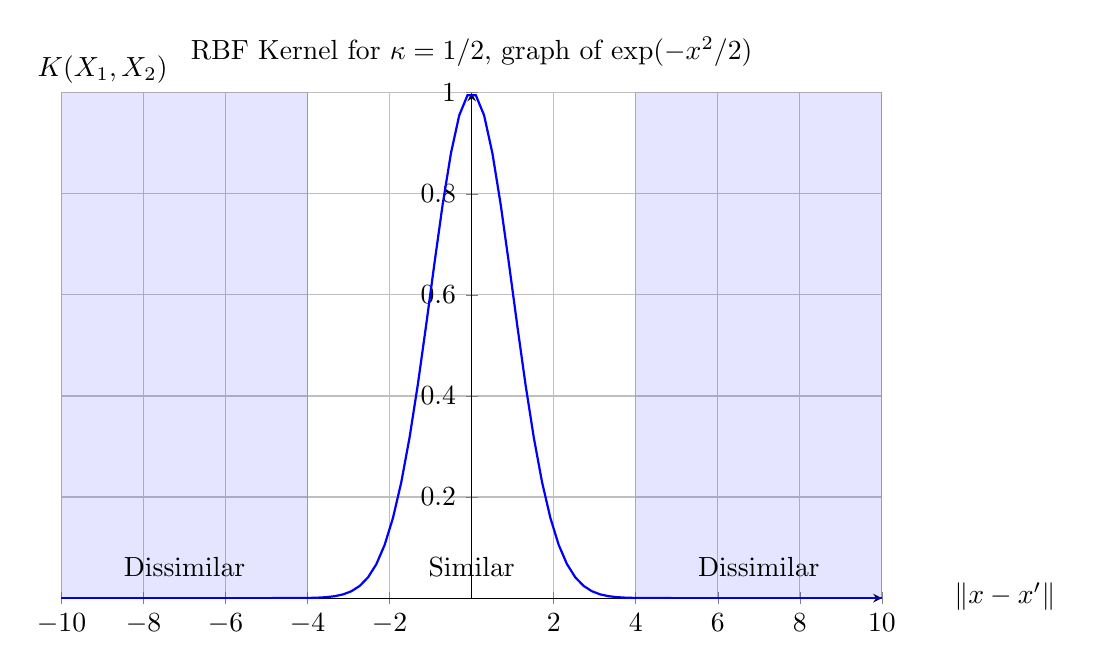
\begin{tikzpicture}
        \begin{axis}[
                width=12cm,
                height=8cm,
                xlabel={$\|x - x'\|$},
                ylabel={$K(X_1, X_2)$},
                grid=major,
                domain=-10:10,
                samples=100,
                xtick={-10,-8,...,10},
                ytick={0,0.2,...,1},
                enlargelimits=false,
                legend pos=outer north east,
                axis lines=middle,
                xlabel style={at={(axis description cs:1.15,0.05)},anchor=north},
                ylabel style={at={(axis description cs:0.05,1)},anchor=south},
                title={RBF Kernel for $\kappa = 1/2$, graph of $\exp(-x^2/2)$},
                ymin=0, ymax=1,
                xmin=-10, xmax=10
            ]
            \addplot [
                blue,
                thick,
                domain=-10:10,
            ]
            {exp(-x^2/2)};

            % Highlight regions
            \draw [fill=blue, opacity=0.1] (axis cs:-10,0) rectangle (axis cs:-4,1);
            \draw [fill=blue, opacity=0.1] (axis cs:4,0) rectangle (axis cs:10,1);

            % Add region labels
            \node at (axis cs:-7,0.1) [anchor=north] {Dissimilar};
            \node at (axis cs:7,0.1) [anchor=north] {Dissimilar};
            \node at (axis cs:0,0.1) [anchor=north] {Similar};

        \end{axis}
    \end{tikzpicture}
    \caption{RBF Kernel for $\kappa = 1/2$, graph of $\exp(-x^2/2)$. Areas of dissimilarity are subjectively noted where the kernel values are negligible.}
    \label{fig:rbf_kernel}
\end{figure}

The RBF kernel is actually a special case of the polynomial basis expansion, where


\subsection{Example Radial Basis Function Kernel}
Given a one-dimensional domain and a one-dimensional co-domain, we have the model $\hat{y} = \phi(x)^\top \theta$.

\begin{equation}
    \phi(x) = \exp(-\gamma ||x - x'||^2) \quad \phi(x) : \mathbb{R}^1 \rightarrow \mathbb{R}^1
\end{equation}

and with a new set of corresponding weights, we have:

\begin{equation}
    \hat{y} = \exp(-\gamma ||x - x'||^2) \cdot \begin{bmatrix} \theta_0 \\ \theta_1 \end{bmatrix} = \theta_0 \exp(-\gamma ||x - x'||^2) + \theta_1
\end{equation}


\section{Linear Algebra}
\subsection{Vectors}

A vector is defined by a list of numbers. It is most useful to geometrically interpret vectors as points in space.

\begin{equation}
    \mb{x} := \begin{bmatrix} x_1 \\ x_2 \\ \vdots \\ x_n \end{bmatrix}
\end{equation}

We have several vector operations:
\begin{itemize}
    \item \textbf{Scalar Multiplication}:
          \begin{equation}
              \alpha \mb{x} = \begin{bmatrix} \alpha x_1 \\ \alpha x_2 \\ \vdots \\ \alpha x_n \end{bmatrix}
          \end{equation}

    \item \textbf{Vector Addition}:
          \begin{equation}
              \mb{x} + \mb{y} = \begin{bmatrix} x_1 + y_1 \\ x_2 + y_2 \\ \vdots \\ x_n + y_n \end{bmatrix}
          \end{equation}

    \item \textbf{Dot Product}:
          \begin{equation}
              \mb{x} ^\top \mb{y} = \sum^n_{i=1} x_i y_i
          \end{equation}
\end{itemize}



\subsection{Matrices}

Matrices define linear transforms. Geometrically, it is best to interpret them as transformations whose columns are the new basis vectors.

\begin{equation}
    \mb{A} := \begin{bmatrix} A_{1,1} & A_{1,2} & \cdots & A_{1,n} \\ A_{2,1} & A_{2,2} & \cdots & A_{2,n} \\ \vdots & \vdots & \ddots & \vdots \\ A_{m,1} & A_{m,2} & \cdots & A_{m,n} \end{bmatrix} \quad \mb{A} \in \mathbb{R}^{m \times n}
\end{equation}


Non-square matrices can be thought of as transformations from $\mathbb{R}^m$ dimentional space to $\mathbb{R}^n$ dimensional space.

\subsection{Matrix Operations}

We define several matrix operations as follows:

\begin{itemize}
    \item \textbf{Scalar Multiplication}:
          \begin{equation}
              cA = c A_{i,j}
          \end{equation}

    \item \textbf{Hadamard Product (Element-wise Multiplication)}:
          \begin{equation}
              A \circ B = A_{i,j} B_{i,j}
          \end{equation}

    \item \textbf{Matrix Subtraction}:
          \begin{equation}
              A - B = A_{i,j} - B_{i,j}
          \end{equation}

    \item \textbf{Matrix Product}:
          \begin{equation}
              C_{i,j} = \sum_{k} A_{i,k} B_{k,j}
          \end{equation}

    \item \textbf{Trace of a Matrix}:
          \begin{equation}
              \text{Tr}(A) = \sum_{i} A_{i,i}
          \end{equation}
\end{itemize}

\textbf{Dimensional Notation}:
\begin{equation}
    A \in \mathbb{R}^{n \times m} : \mathbb{R}^n \to \mathbb{R}^m
\end{equation}
\begin{equation}
    B \in \mathbb{R}^{m \times k} : \mathbb{R}^m \to \mathbb{R}^k
\end{equation}
\begin{equation}
    AB \in \mathbb{R}^{n \times k} : \mathbb{R}^n \to \mathbb{R}^k
\end{equation}



\sn{Matrix Multiplication as Dot Products of the Row and Column}{
    This matrix multiplication is equivalent to the dot product between row \( i \) of matrix \( A \) and column \( j \) of matrix \( B \):
    \begin{equation}
        \mb{x}^\top \mb{y} = \sum_{i=1}^{n} x_i y_i
    \end{equation}
}


\subsection{Einstein/Pythonic Index Notation}
\marginnote{Refer to this \href{https://www.youtube.com/watch?v=CLrTj7D2fLM}{video on Einstein summation convention} for more information.}
\hl{Most readers will have covered a lot of the linear algebra basics before, if so, this is the most important section to read!}
As reasoning about matrix and vector products can sometimes be cumbersome, it is often useful to write out the operations we perform in index notation. The matrix product $C = AB$ can be written as: $C_{i,j} = \sum_k A_{i,k}B_{k,j}$. It can also be useful to adopt a more ``pythonic" index notation where we consider the system $Ax = b$ and write the first entry of the vector $b$ as:


\begin{equation}
    A_{1,:}x = b_1
\end{equation}
which indicates that the first value of the result is simply the dot product of the first row of matrix $A$ with the vector $x$.

Then, we can write the entire system as:
\begin{equation}
    C_{i,j} = \sum A_{i,:}B_{:,j}
\end{equation}




Generally in tensor calculus, a lot of expressions involve summing over particular indices.

\begin{equation}
    \sum^3_{i=1} a_i x_i = a_1 x_1 + a_2 x_2 + a_3 x_3
\end{equation}

\marginnote{\extrasb{Fun fact}{Yes, this was introduced by Albert Einstein in 1916!}}
In \textbf{Einstein notation}, we can write this as:
\begin{equation}
    a_i x_i \quad (i = 1,2,3)
\end{equation}

This brings us to our first rule (and several others):
\begin{enumerate}[label=\textbf{Rule \arabic*}:, leftmargin=*, labelsep=1em]
    \item Any twice-repeated index in a single term is implicitly summed over. Typically, this is from index 1 to 3 because most calculations are done in 3D space. For example, if we had:
          \begin{equation}
              a_{ij} b_{j} = a_{i1}b_1 + a_{i2}b_2 + a_{i3}b_3
          \end{equation}

          We can then express this in the Einstein notation as:
          \begin{equation}
              a_{ij} b_{j} = a_{i\alpha} b_\alpha \quad \alpha \in \{1,2,3\}
          \end{equation}
          This will begin to make more sense as we come up with a better way to describe indices that appear once, and twice-repeated indices.

    \item The definitions of indices:
          \begin{itemize}
              \item We let $j$ be the dummy index, because it is repeated only twice. One can thus replace $j$ with any other index or letter, it is just a placeholder (thus called a dummy index). Although more rigorously:
                    \begin{itemize}
                        \item One can replace any dummy index with a letter/index that is not already used in the expression.
                        \item This letter must be over the same range as the original dummy index, so in the case of replacing $j$, it must be over the range 1 to 3.
                    \end{itemize}
                    \begin{align}
                        a_{ij} b_{j} & = a_{i1}b_1 + a_{i2}b_2 + a_{i3}b_3               \\
                                     & = a_{i\alpha} b_\alpha \quad \alpha \in \{1,2,3\}
                    \end{align}
              \item $i$ is the free index, which can take on any value that $j$ takes on, but it is not summed over and can only take on one value at a time $i \in \{1,2,3\}$.
              \item The free index occurs only \textbf{once} in the expression and \textbf{cannot be replaced by another free index,}
                    \begin{equation}
                        a_{ij} b_{j} \neq a_{kj} b_{j}
                    \end{equation}
              \item To help avoid confusion, one tip is to use roman letters ($i$, $j$, $k$) for free indices, and greek letters ($\lambda$, $\mu$, $\rho$) for dummy indices.

          \end{itemize}
    \item No index may occur 3 or more times in a given term.
          \begin{itemize}
              \item $a_{ij}b_{ij}\quad \checkmark$
              \item $a_{ii}b_{ij}\quad \times$
              \item $a_{ij}b_{ij}\quad \times$
              \item $a_{ij}b_{j} + a_{ji}b_{j} \quad \checkmark$
          \end{itemize}
          In the last example, we are adding \textbf{multiple terms}, so the index occurence rule only applies by term. So $j$ is a dummy index for both terms since it occurs twice (per term).
    \item In an equation involving Einstein notation, the free indices on the left-hand side must match the right-hand side.
          \begin{itemize}
              \item $x_i = a_{ij}b_j \quad \checkmark$
                    \begin{itemize}
                        \item $i$ is a free index on both the LHS and RHS.
                    \end{itemize}

              \item $a_i = A_{xi}B_{xk} x_j + C_{ik}u_k \quad \checkmark$
                    \begin{itemize}
                        \item $i$ is the free index on both the LHS and RHS.
                    \end{itemize}

              \item $x_i = A_{ij} \quad \times$
                    \begin{itemize}
                        \item $i$ is a free index on both the LHS and RHS, but $j$ is a free index on the RHS that is not on the LHS.
                    \end{itemize}

              \item $x_j = A_{ik}u_k \quad \times$
                    \begin{itemize}
                        \item LHS free index: $j$.
                        \item RHS free index: $i$.
                    \end{itemize}

              \item $x_i = A_{ik}u_k + c_j \quad \times$
                    \begin{itemize}
                        \item LHS free index: $i$.
                        \item RHS free indices: $i$ and $j$.
                    \end{itemize}
          \end{itemize}
\end{enumerate}


\textbf{Relating Einstein Notation to Pythonic Notation}:
We had:
\begin{equation}
    C_{i,j} = \sum_k A_{i,k}B_{k,j}
\end{equation}

Since $k$ is our dummy variable (it is summed over and doesn't appear in the final result), we can replace it with colon (:) to indicate we are working with all elements along that dimension. So we have

\begin{equation}
    C_{i,j} = A_{i,:}B_{:,j}
\end{equation}

In Python, this is:
\begin{lstlisting}[
    language=Python,
    basicstyle=\ttfamily\small,  % Monospace with smaller font
    keywordstyle=\bfseries\color{blue},  % Bold keywords, coloured blue
    commentstyle=\itshape\color{green!50!black},  % Italic comments, dark green
    stringstyle=\color{red},  % Strings in red
    numberstyle=\tiny,  % Line numbers in small font
    frame=single,  % Add a frame around the code
  ]
C[i, j] = np.dot(A[i, :], B[:, j])
\end{lstlisting}


% \begin{itemize}
%     \item Free indices appear only once in an expression and thus are not summed over. Dummy indices appear twice, and are implicitly summed over.
%     \item To help avoid confusion, use roman letters ($i$, $j$, $k$) for free indices, and greek letters ($\lambda$, $\mu$, $\rho$) for dummy indices.
%     \item Dummy indices should never appear in the final answer.
%     \item The free indices should always be the same in every term in an expression.
%     \item An index should never appear more than twice in a single term.
% \end{itemize}



\subsection{Matrix Properties: Linear Dependence}

Two vectors are said to be \textbf{linearly dependent} if one is a scalar multiple of the other. That is, for vectors \( \mb{a} \) and \( \mb{b} \), we have:
\begin{equation}
    \mb{a} = \alpha \mb{b}
\end{equation}
where \( \alpha \in \mathbb{R} \) is a scalar.

A set of vectors \( \{ \mb{a}^{(1)}, \mb{a}^{(2)}, \dots, \mb{a}^{(n)} \} \) is linearly dependent if there exist non-zero real weights \( v^{(i)} \) such that their weighted sum results in the zero vector:
\begin{equation}
    v^{(1)} \mb{a}^{(1)} + \dots + v^{(n)} \mb{a}^{(n)} = 0
\end{equation}
This implies that at least one vector in the set can be written as a linear combination of the others:
\begin{equation}
    \mb{a}^{(1)} = - \frac{v^{(2)}}{v^{(1)}} \mb{a}^{(2)} - \dots - \frac{v^{(n)}}{v^{(1)}} \mb{a}^{(n)}
\end{equation}

\subsection{Span of Vectors}

The \textbf{span} of a set of vectors \( \{ \mb{v}^{(i)} \}_{i=1}^{K} \) is the set of all possible linear combinations of these vectors. Formally, the span is given by:
\begin{equation}
    \text{Span}(V) = \left\{ \sum_{i=1}^{K} \lambda^{(i)} \mb{v}^{(i)} \mid \lambda^{(i)} \in \mathbb{R} \right\}
\end{equation}
Here, the coefficients \( \lambda^{(i)} \) are real numbers, and the span defines the vector subspace formed by these linear combinations.

\subsection{From Span to Rank}

The \textbf{rank} of a matrix \( A \), formed by stacking column vectors \( \mb{a}^{(1)}, \dots, \mb{a}^{(K)} \), is the dimension of the vector space spanned by these vectors. If:
\begin{equation}
    A = \begin{bmatrix} \mb{a}^{(1)\top} & \cdots & \mb{a}^{(K)\top} \end{bmatrix}
\end{equation}
Then:
\begin{equation}
    \text{Rank}(A) = \text{Span}\left( \mb{a}^{(1)\top}, \dots, \mb{a}^{(K)\top} \right)
\end{equation}
A matrix is said to be \textbf{full rank} if the rank of the matrix equals the number of its rows or columns (i.e., if an \( n \times n \) matrix has rank \( n \)).

\subsection{Eigen Decomposition}

Given a matrix \( A \in \mathbb{R}^{n \times n} \), an \textbf{eigenvector} \( \mb{v} \) and an \textbf{eigenvalue} \( \lambda \) satisfy the following equation:
\begin{equation}
    A \mb{v} = \lambda \mb{v}
\end{equation}

Note that any scalar multiple of \( \mb{v} \) is also an eigenvector. To standardise, we typically normalise the eigenvector to have unit length:
\begin{equation}
    \| \mb{v} \|_2 = 1
\end{equation}
This ensures that the eigenvector is unique up to a scalar factor.

\subsection{Eigen Decomposition of a Matrix}

The \textbf{eigen decomposition} of a matrix \( A \in \mathbb{R}^{n \times n} \) expresses the matrix in terms of its eigenvalues and eigenvectors. Formally, this decomposition is given by:
\begin{equation}
    A = Q \Lambda Q^{-1}
\end{equation}
where:
\begin{itemize}
    \item \( Q \) is the matrix whose columns are the eigenvectors of \( A \).
    \item \( \Lambda \) is a diagonal matrix with the eigenvalues \( \lambda_i \) of \( A \) on the diagonal.
\end{itemize}
The eigen decomposition allows us to express \( A \) as a product of its eigenvectors and eigenvalues, enabling many applications in linear algebra, such as simplifying powers of matrices or solving systems of linear equations.

\subsection{Norms}

\begin{marginfigure}
    \centering
    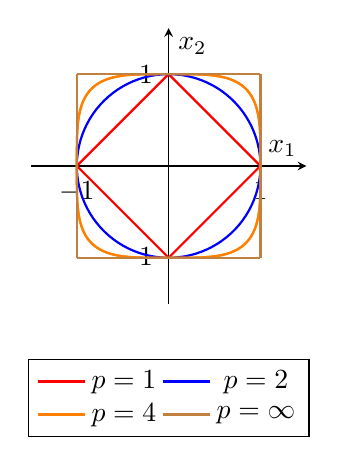
\begin{tikzpicture}
        \begin{axis}[
                axis lines=middle,
                xlabel=\(x_1\),
                ylabel=\(x_2\),
                xmin=-1.5, xmax=1.5,
                ymin=-1.5, ymax=1.5,
                axis equal image,
                legend style={at={(0.5,-0.2)},anchor=north,legend columns=2}, % Move legend below
                width=2in,
                height=2in
            ]

            % Legend entries
            \addlegendimage{red, thick}
            \addlegendentry{\(p=1\)}
            \addlegendimage{blue, thick}
            \addlegendentry{\(p=2\)}
            \addlegendimage{orange, thick}
            \addlegendentry{\(p=4\)}
            \addlegendimage{brown, thick}
            \addlegendentry{\(p=\infty\)}

            % 1-norm (diamond shape)
            \addplot [red, thick, domain=-1:1, samples=100] ({1-abs(x)},x);
            \addplot [red, thick, domain=-1:1, samples=100] ({-1+abs(x)},x);

            % 2-norm (circle)
            \addplot [blue, thick, domain=0:360, samples=100] ({cos(x)},{sin(x)});

            % 4-norm
            \addplot [orange, thick, domain=0:360, samples=100, variable=\t]
            ({(cos(t)^(4) + sin(t)^(4))^(-1/4)*cos(t)}, {(cos(t)^(4) + sin(t)^(4))^(-1/4)*sin(t)});
            \addplot [orange, thick, domain=0:360, samples=100, variable=\t]
            ({-(cos(t)^(4) + sin(t)^(4))^(-1/4)*cos(t)}, {-(cos(t)^(4) + sin(t)^(4))^(-1/4)*sin(t)});

            % Infinity norm (square)
            \addplot [brown, thick, domain=-1:1] ({1},x);
            \addplot [brown, thick, domain=-1:1] ({-1},x);
            \addplot [brown, thick, domain=-1:1] (x,{1});
            \addplot [brown, thick, domain=-1:1] (x,{-1});

        \end{axis}
    \end{tikzpicture}
    \caption{Different norms in 2D space.}
    \label{fig:norms}
\end{marginfigure}
A \textbf{norm} is a function that assigns a non-negative length or size to a vector. Norms are widely used in mathematics to measure distances or lengths in vector spaces. Below are some commonly used norms:

\begin{itemize}
    \item \textbf{Euclidean Norm (2-norm)}: Also known as the straight-line distance, the Euclidean norm is given by:
          \begin{equation}
              \| \mb{x} \|_2 = \sqrt{\sum_i x_i^2}
          \end{equation}

    \item \textbf{p-norm}: The \( p \)-norm generalises the Euclidean norm to other values of \( p \):
          \begin{equation}
              \| \mb{x} \|_p = \left( \sum_i |x_i|^p \right)^{1/p}
          \end{equation}
          Special cases of the \( p \)-norm include:
          \begin{itemize}
              \item The 2-norm (Euclidean norm) when \( p = 2 \).
              \item The 1-norm, which represents the Manhattan distance, when \( p = 1 \).
          \end{itemize}

    \item \textbf{Zero Norm (Hamming Distance)}: The 0-norm counts the number of non-zero elements in a vector:
          \begin{equation}
              \| \mb{x} \|_0 = \sum_i \mathbb{I}(x_i \neq 0)
          \end{equation}
          where \( \mathbb{I}(\cdot) \) is the indicator function, which returns 1 if the condition is true and 0 otherwise.

    \item \textbf{Infinity Norm}: Also called the \textit{supremum norm}, the infinity norm is defined as the largest absolute value among the vector components:
          \begin{equation}
              \| \mb{x} \|_\infty = \sup_n |x_n|
          \end{equation}

    \item \textbf{Mahalanobis Distance}: The Mahalanobis distance takes into account the correlations between variables in a dataset:
          \begin{equation}
              d_S(\mb{x}, \mb{y}) = (\mb{x} - \mb{y})^T S (\mb{x} - \mb{y})
          \end{equation}
          where \( S \) is a positive semi-definite matrix, typically the covariance matrix of the data.

\end{itemize}



Norms are typically used as a way to measure distances and magnitudes.

\thm{Geometric Interpretation of the Mahalanobis Distance}{
    Given a positive semi-definite matrix \( S \in \mathbb{R}^{m \times m} \), a feature vector \( \mathbf{x'} \in \mathbb{R}^m \), and a similarity threshold \( \delta \), all vectors \( \mathbf{x''} \in \mathbb{R}^n \) satisfying \( d_S(\mathbf{x'}, \mathbf{x''}) \leq \delta \) are contained within the axis-aligned orthotope:
    \[
        [\mathbf{x'} - \delta \sqrt{\mathbf{d}}, \mathbf{x'} + \delta \sqrt{\mathbf{d}}]
    \]
    where \( \mathbf{d} = \text{diag}(S) \), the vector containing the elements along the diagonal of \( S \).
}

\subsection{Equivalence of Inner Product and Euclidean Norm}

We aim to prove the equivalence between the quadratic form and the squared Euclidean norm:
\begin{equation}
    \text{Claim: }(\theta^T \mathbf{X} - \mathbf{y})^T (\theta^T \mathbf{X} - \mathbf{y}) = \| \theta^T \mathbf{X} - \mathbf{y} \|_2^2
\end{equation}

\textbf{Left-hand side (LHS):} The quadratic form on the LHS can be expanded as:

\begin{align}
    (\theta^T \mathbf{X} - \mathbf{y})^T (\theta^T \mathbf{X} - \mathbf{y}) & = \left( \left( \sum_i \theta_i^\top \mathbf{X}_{i,j} \right) - \mathbf{y}_j \right)^\top \left( \left( \sum_i \theta_i^\top \mathbf{X}_{i,j} \right) - \mathbf{y}_j \right)         \\
                                                                            & = \sum_j \left( \left( \sum_i \theta_i^\top \mathbf{X}_{i,j} \right) - \mathbf{y}_j \right) ^\top \left( \left( \sum_i \theta_i^\top \mathbf{X}_{i,j} \right) - \mathbf{y}_j \right) \\
                                                                            & = \sum_j \left( \left( \sum_i \theta_i^\top \mathbf{X}_{i,j} \right) - \mathbf{y}_j \right)^2
\end{align}

\bigskip

\textbf{Right-hand side (RHS):} The squared Euclidean norm is defined as:

\begin{equation}
    \| \theta^T \mathbf{X} - \mathbf{y} \|_2^2
\end{equation}

We know that the Euclidean norm is given by:
\begin{equation}
    \| \mathbf{x} \|_2 = \sqrt{\sum_i x_i^2}
\end{equation}

Therefore, we expand into:
\begin{align}
    \| \theta^T \mathbf{X} - \mathbf{y} \|_2^2 & = \left( \sqrt{\sum_j \left( \sum_i \theta_i^T \mathbf{X}_{i,j} - \mathbf{y}_j \right)^2} \right)^2 \\
                                               & = \sum_j \left( \sum_i \theta_i^T \mathbf{X}_{i,j} - \mathbf{y}_j \right)^2
\end{align}


\bigskip

\textbf{Conclusion:} Both the LHS and RHS are equivalent, as they both expand into the same form:

\begin{equation}
    \sum_j \left( \sum_i \theta_i^T \mathbf{X}_{i,j} - \mathbf{y}_j \right)^2
\end{equation}

This shows that the inner product expression for \( (\theta^T \mathbf{X} - \mathbf{y})^T (\theta^T \mathbf{X} - \mathbf{y}) \) is equivalent to the squared Euclidean norm \( \| \theta^T \mathbf{X} - \mathbf{y} \|_2^2 \), confirming the claim.
\bigskip

To finish it off in index notation, this is written as:
\begin{equation}
    \theta_i \mb{X}_{i,j}
\end{equation}

\section{Revisiting Calculus}

Recall from your previous studies that the derivative of a real-valued function \( f(x) \) is defined as the limit of the difference quotient:
\begin{equation}
    f'(x) = \frac{df}{dx} = \lim_{h \to 0} \frac{f(x+h) - f(x)}{h}
\end{equation}

This limit definition is important to understanding how functions change locally around a particular point. While differentiation can sometimes be difficult to compute directly, this formula also provides a method for approximating the derivative numerically. For any interested reader, the method of zeroth-order optimisation can be explored for more computational approaches.

Several useful derivatives of common functions include:
\begin{align*}
    f(x) & = x^n,      & f'(x) & = n x^{n-1}      \\
    f(x) & = \sin(x),  & f'(x) & = \cos(x)        \\
    f(x) & = \tanh(x), & f'(x) & = 1 - \tanh^2(x) \\
    f(x) & = \exp(x),  & f'(x) & = \exp(x)        \\
    f(x) & = \log(x),  & f'(x) & = \frac{1}{x}
\end{align*}

It is important to recall the key rules of differentiation that allow us to easily compute derivatives of more complex expressions. These rules are essential for differentiating composite functions and will be useful throughout the course.

\subsection{Sum Rule}
The derivative of the sum of two functions is given by:
\begin{equation}
    (f(x) + g(x))' = f'(x) + g'(x) = \frac{df(x)}{dx} + \frac{dg(x)}{dx}
\end{equation}

\subsection{Product Rule}
The derivative of the product of two functions is given by:
\begin{equation}
    (f(x)g(x))' = f'(x)g(x) + f(x)g'(x) = \frac{df(x)}{dx} g(x) + f(x) \frac{dg(x)}{dx}
\end{equation}

\subsection{Chain Rule}
The derivative of the composition of two functions is given by:
\begin{equation}
    (g \circ f)'(x) = (g(f(x)))' = g'(f(x)) f'(x) = \frac{dg(f(x))}{df} \frac{df(x)}{dx}
\end{equation}

\subsection{Quotient Rule}
The derivative of the quotient of two functions is given by:
\begin{equation}
    \left( \frac{f(x)}{g(x)} \right)' = \frac{f'(x)g(x) - f(x)g'(x)}{(g(x))^2} = \frac{\frac{df(x)}{dx} g(x) - f(x) \frac{dg(x)}{dx}}{(g(x))^2}
\end{equation}

These rules will be useful as we move forward and encounter more complex functions to differentiate.

\section{Gradients and Partial Derivatives}

The derivative can be generalised for functions \( f : \mathbb{R}^n \to \mathbb{R} \), where \( f(x) \) depends on multiple variables \( x_1, x_2, \dots, x_n \). We compute the \textbf{partial derivative} with respect to each variable by holding the others constant:
\begin{equation}
    \frac{\partial f}{\partial x_1} = \lim_{h \to 0} \frac{f(x_1 + h, x_2, \dots, x_n) - f(x_1, x_2, \dots, x_n)}{h}
\end{equation}

We collect these partial derivatives into the \textbf{gradient vector}:
\begin{equation}
    \nabla f = \left[ \frac{\partial f}{\partial x_1}, \frac{\partial f}{\partial x_2}, \dots, \frac{\partial f}{\partial x_n} \right]
\end{equation}

When dealing with vector-valued functions \( f : \mathbb{R}^n \to \mathbb{R}^m \), the gradient generalises to the \textbf{Jacobian matrix} \( \nabla f \in \mathbb{R}^{m \times n} \):
\begin{equation}
    \nabla f = \begin{bmatrix}
        \frac{\partial f_1}{\partial x_1} & \frac{\partial f_1}{\partial x_2} & \cdots & \frac{\partial f_1}{\partial x_n} \\
        \frac{\partial f_2}{\partial x_1} & \frac{\partial f_2}{\partial x_2} & \cdots & \frac{\partial f_2}{\partial x_n} \\
        \vdots                            & \vdots                            & \ddots & \vdots                            \\
        \frac{\partial f_m}{\partial x_1} & \frac{\partial f_m}{\partial x_2} & \cdots & \frac{\partial f_m}{\partial x_n}
    \end{bmatrix}
\end{equation}

For functions \( f: \mathbb{R}^{n \times m} \to \mathbb{R}^{k \times l} \), the gradient forms a tensor of shape \( (k \times l) \times (n \times m) \), where each element represents the partial derivative of an output with respect to an input variable.

\subsection{Vector Calculus Identities to Remember}

Below are some key vector calculus identities that will prove useful in various contexts:

\begin{align*}
     & \frac{\partial \bm{x}^\top \bm{a}}{\partial \bm{x}}                             & = & \quad\bm{a}^\top                                                               \\
     & \frac{\partial}{\partial \bm{X}} f(\bm{X})^\top                                 & = & \quad\left( \frac{\partial f(\bm{X})}{\partial \bm{X}} \right)^\top            \\
     & \frac{\partial}{\partial \bm{X}} \text{tr}(f(\bm{X}))                           & = & \quad\text{tr} \left( \frac{\partial f(\bm{X})}{\partial \bm{X}} \right)       \\
     & \frac{\partial}{\partial \bm{X}} f(\bm{X})^{-1}                                 & = & \quad-f(\bm{X})^{-1} \frac{\partial f(\bm{X})}{\partial \bm{X}} f(\bm{X})^{-1} \\
     & \frac{\partial \bm{a}^\top \bm{Xb}}{\partial \bm{X}}                            & = & \quad\bm{a} \bm{b}^\top                                                        \\
     & \frac{\partial}{\partial s} (\bm{x} - \bm{A} s)^\top \bm{W} (\bm{x} - \bm{A} s) & = & \quad-2 (\bm{x} - \bm{A}s)^\top \bm{W} \bm{A}
\end{align*}

\section{Error Optimisation}
\subsection{Minimal Optimization Formulation}
Given the discussion of basis expansion, we can write a more general version of linear regression (including an expanded basis) as:
\begin{equation}
    \hat{y}^{(i)} = \phi(x^{(i)})^T \theta
\end{equation}
The critical learning question in this model is how do we pick the best $\theta$?
Unfortunately, outside of linear models, this question does not always have a straight-forward answer and depends on several critical modelling decisions. However, for now, we will take the most basic approach, which is the standard, frequentist learning approach. This is where we model the "best" $\theta$ as the one that minimizes a loss or error function, $\mathcal{L}$.

\subsection{Loss Function}

One such loss function is:

\begin{equation}
    \mathcal{L}(y^{(i)}, \hat{y}^{(i)}) = ||y^{(i)} - \hat{y}^{(i)}||_2^2
\end{equation}

This is known as the $\ell_2$ or mean squared error loss. We can write down learning in the linear regression model as the following optimisation problem:

\begin{equation}
    \arg\min_{\theta} [\mathbb{E}_{(x,y)\sim\mathcal{D}}[\mathcal{L}(y, \hat{y})]]
\end{equation}

That is, the best $\theta$ is the value of $\theta$ that minimizes the expected loss. Notice that though $\theta$ does not appear in the above equation, $\hat{y}$ depends directly on $\theta$.

\subsection{Learning in a Linear Model}

In a linear model, we can express the loss function as:

\begin{equation}
    \mathcal{L}(\hat{y}_i, y_i) = (\hat{y}_i - y_i)^2
\end{equation}

\begin{equation}
    \mathcal{L}(\theta) = \frac{1}{N} \left( ||\theta^T X - y||_2^2 \right)
\end{equation}

Our optimisation problem becomes:

\begin{equation}
    \arg\min_{\theta} \mathcal{L}(\theta)
\end{equation}

Note: We can drop the $\frac{1}{N}$ factor because we care about finding the argmin, not the min itself.

\subsection{Deriving the Optimal Parameter Value}

To find the optimal parameter value, we can derive the loss function with respect to $\theta$ and set it to zero:

\begin{equation}
    \mathcal{L}(\theta) = (\theta^T X - y)^T (\theta^T X - y)
\end{equation}

\begin{equation}
    \nabla_\theta (\theta^T X - y)^T (\theta^T X - y) = 0
\end{equation}

Simplifying:

\begin{equation}
    \nabla_\theta ||\theta^T X - y||_2^2 = -2X^T (y - \theta^T X)
\end{equation}

\begin{equation}
    -2X^T (y - \theta^T X) = 0
\end{equation}

\begin{equation}
    X^T y - X^T X \theta^T = 0
\end{equation}

\begin{equation}
    X^T y = X^T X \theta^T
\end{equation}

Finally, we arrive at the solution:

\begin{equation}
    (X^T X)^{-1} X^T y = \theta^T
\end{equation}

This gives us the optimal parameter value for the linear regression model.
\bigskip

What about non-linear models? That's another story...
